%% Copyright (C) 2019 Turysaz, Bitbonk

%% Copyright (C) 2019 Turysaz, Bitbonk

\usepackage[utf8]{inputenc}
\usepackage[T1]{fontenc}
\usepackage[english]{babel}

\usepackage{todonotes}

%% packages needed by DarkConsole theme
\usepackage{xcolor}
\usepackage{pgf}
\usepackage{droidsans}
\usepackage{fvextra}
\usepackage{upquote}
\usepackage{slantsc}
%\usepackage{minted} %% needs shell escaping...
%\usepackage{ifplatform} %% needs shell escaping...
\usepackage{xstring}
\usepackage{framed}

\usetheme{DarkConsole}

\usepackage{pdfpcnotes}

\usepackage{caption}
\captionsetup[figure]{labelformat=empty}

\newcommand{
    \emojiLarge}[1]{
    \includegraphics[width=2cm]{../3rd-party/coloremoji/emoji_images/hires/#1.pdf}}

\newcommand{
    \emojiMedium}[1]{
    \includegraphics[width=1cm]{../3rd-party/coloremoji/emoji_images/hires/#1.pdf}}


\newcommand{
    \emojiSmall}[1]{
    \includegraphics{../3rd-party/coloremoji/emoji_images/hires/#1.pdf}}

\newcommand{\emojiCheck}{\emojiSmall{2705}}
\newcommand{\emojiFail}{\emojiSmall{1F6AB}}

%\newcommand{\says}[1]{\note{\huge{Says: \alert{#1}}}}
\newcommand{\says}[1]{\pnote{Says: #1}}



%% variables for koma title page
\author{\{@turysaz, @bitbonk\}}
\title{\Huge{Knit Rider}\\
    \large{Bring that 80s knitting machine to the \mbox{21st century}!}
}

\date{\today{}}

\begin{document}

\maketitle

\begin{frame}{init}
    \says{bitbonk}
    So we had an old knitting machine...
\end{frame}

\begin{frame}{overview}
    \says{bitbonk}
    \begin{figure}
        \includegraphics[width=1\textwidth]{./images/foto-overview.jpg}
    \end{figure}
\end{frame}

\begin{frame}{needles}
    \says{bitbonk}
    \begin{figure}
        \includegraphics[width=0.5\textwidth]{./images/foto-nadelbett.jpg}
    \end{figure}
\end{frame}

\begin{frame}{slay}
    \says{bitbonk}
    \begin{figure}
        \includegraphics[width=0.8\textwidth]{./images/foto-slay.jpg}
    \end{figure}
\end{frame}

\begin{frame}{keypad}
    \says{bitbonk}
    \begin{figure}
        \includegraphics[width=0.8\textwidth]{./images/foto-computer.jpg}
    \end{figure}
\end{frame}

\begin{frame}{patterns}
    \says{bitbonk}
    \begin{figure}
        \includegraphics[width=0.5\textwidth]{./images/foto-muster.jpg}
    \end{figure}
\end{frame}

\begin{frame}{patterns}
    \says{bitbonk}
    \begin{figure}
        \includegraphics[width=0.5\textwidth]{./images/foto-muster-2.jpg}
    \end{figure}
\end{frame}

\begin{frame}{init}
    \says{bitbonk}
    ...but the best thing is...\pause
    \begin{figure}
        \includegraphics[width=0.4\textwidth]{./images/foto-serial-interface.jpg}
        \caption{it has a serial interface \emojiMedium{1F631}}
    \end{figure}
\end{frame}

\begin{frame}{computer}
    \says{bitbonk}
    \begin{figure}
        \includegraphics[width=0.5\textwidth]{./images/foto-why-computer.jpg}
    \end{figure}
\end{frame}

\begin{frame}{please not}
    \says{bitbonk}
    \begin{figure}
        \includegraphics[width=0.5\textwidth]{./images/foto-scope.jpeg}
    \end{figure}
\end{frame}

\begin{frame}{the idea}
    \says{bitbonk}
    \begin{enumerate}[<+->]
        \item Take a photo!
        \item Image processing!
        \item Do \_all\_ the soldering!
        \item Speak the protocol!
        \item Knit your face!
    \end{enumerate}
\end{frame}


\begin{frame}{the project architecture}
    \says{bitbonk}
    \begin{figure}
        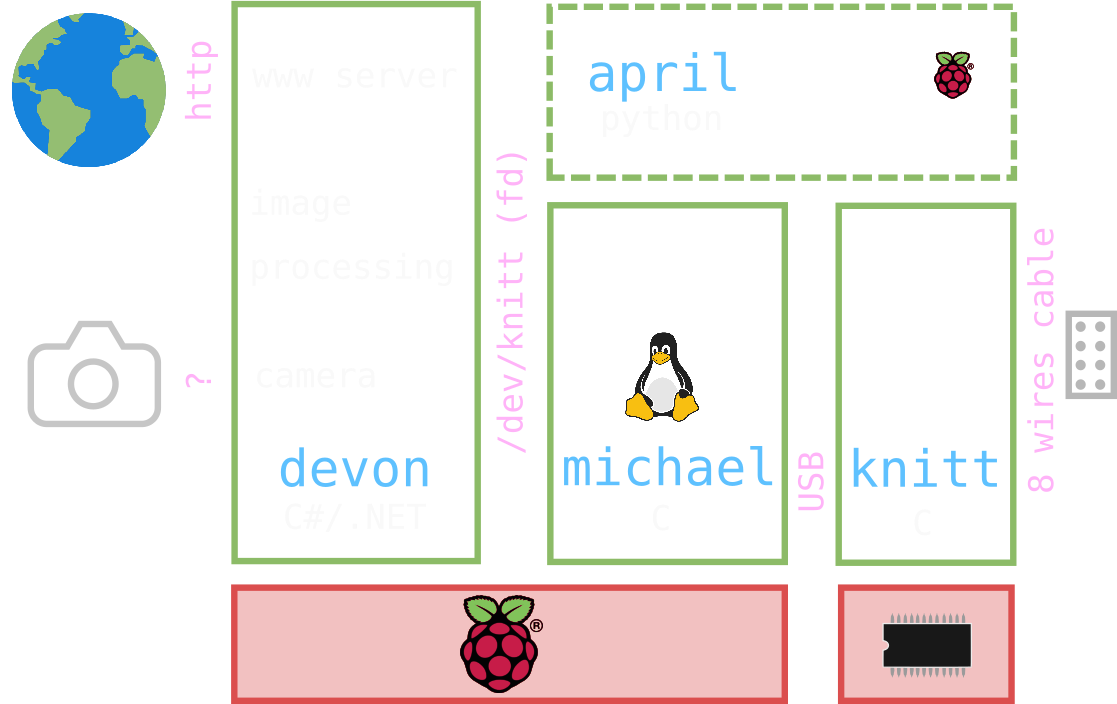
\includegraphics[width=\textwidth]{./images/architecture.png}
    \end{figure}
\end{frame}

\begin{frame}{progress}
    \says{bitbonk}
    \begin{enumerate}
        \item project name \pause \emojiCheck \pause
        \item github repos \pause \emojiCheck \pause
        \item project logo \pause \emojiCheck \pause
        \item usb protocol \pause \emojiCheck \pause
        \item knit manually \pause \emojiCheck \pause
        \item power on ...! \pause
    \end{enumerate}

    \center
    \emojiLarge{1F4A1} \pause %% Light
    \emojiLarge{1F50A} \pause %% Sound
    \emojiLarge{1F4A5} \pause %% Boom
    \emojiLarge{1F525} \pause %% Fire
    \emojiLarge{1F635}        %% Dead
\end{frame}


\begin{frame}{progress}
    \says{bitbonk}
    \begin{figure}
        \includegraphics[width=0.7\textwidth]{./images/fubar.jpg}
        \caption{fubar}
    \end{figure}
\end{frame}

\begin{frame}{progress}
    \says{turysaz}
    \begin{enumerate}
        \item project name \emojiCheck
        \item github repos \emojiCheck
        \item project logo \emojiCheck
        \item usb protocol \emojiCheck
        \item knit manually \emojiCheck
        \item power on ... \emojiFail \pause
        \item repair...
    \end{enumerate}
\end{frame}

\begin{frame}{repairing}
    \says{bitbonk}
    \begin{figure}
        \includegraphics[width=0.4\textwidth]{./images/foto-repair-1.jpg}
    \end{figure}
\end{frame}

\begin{frame}{repairing}
    \says{bitbonk}
    \begin{figure}
        \includegraphics[width=0.8\textwidth]{./images/foto-repair-2.jpg}
    \end{figure}
\end{frame}


\begin{frame}{repairing}
    \says{bitbonk}
    \begin{figure}
        \includegraphics[width=0.8\textwidth]{./images/foto-repair-3.jpg}
    \end{figure}
\end{frame}

\begin{frame}{repairing}
    \says{bitbonk}
    \begin{figure}
        \includegraphics[width=0.5\textwidth]{./images/foto-repair-4-1.jpg}
    \end{figure}
\end{frame}

\begin{frame}{repairing}
    \says{bitbonk}
    \begin{figure}
        \includegraphics[width=0.5\textwidth]{./images/foto-repair-5.jpg}
    \end{figure}
\end{frame}


\begin{frame}{progress}
    \says{turysaz}
    \begin{enumerate}
        \item project name \emojiCheck
        \item github repos \emojiCheck
        \item project logo \emojiCheck
        \item usb protocol \emojiCheck
        \item knit manually \emojiCheck
        \item power on ... \emojiFail
        \item repair... \pause \emojiCheck
    \end{enumerate}
\end{frame}


\begin{frame}{next steps}
    \says{bitbonk}
    \begin{enumerate}
        \item knit more manually
        \item understand protocol better
        \item driver implementation
        \item image processing
    \end{enumerate}
\end{frame}

\end{document}

